\section{Experiments and observed limitations}
\label{sec:adaptive_evaluation}

The experiments evaluate time-adaptive decisions constructed from
historical local-minimum trajectories. Comparisons with pooled
forecast cross-validation are independent out-of-sample benchmarks.
The larger financial and changing-roughness evaluations did not
confirm an unconditional performance improvement.

\subsection{Tracked-minimum evaluation}

The branch experiments recover local minima at historical rolling
origins, connect nearby candidates with a one-to-one correspondence
under a fixed continuation radius, and summarize each branch by
persistence and the subsequent Validation-2 loss. The baseline
historical selector $\psi$ prefers persistent, predictive branches.
Different maps $\phi$ act on the selected branch while sharing the
same numerical candidate recovery, branch identities, and outer
test blocks.

Checkpoint 04 used a four-series development and reserved-confirmation
design. The recency-weighted rule with three-origin half-life was
frozen before evaluating the 16 held-out confirmation blocks.
Checkpoint 05 applied it without retuning to 64 other financial
series, each with four outer blocks. Its broader results motivated
Checkpoint 06, a \emph{post-hoc} analysis of native continuation
stability using earlier blocks from the same series. The order
restriction in that diagnostic is explanatory; it is not a new
external confirmation.

\subsection{Controlled dynamic roughness and the rule family}

Checkpoint 07 fixes $d=2$ and studies 1,200 simulated scenarios with
constant, gradually changing, or abruptly switching latent
slope-innovation variance, using 100 seeds and two observation-noise
scales. It provides a controlled comparison between the pooled
selector, the newest local minimum, and recency averaging along a
tracked branch.

Checkpoint 08 uses a disjoint set of 100 seeds and the same family
of roughness mechanisms. It fixes the underlying branch selection
while evaluating several maps $\phi$, including linear trends fitted
to recent smoothness values, exponentially weighted linear trends,
and weighted increments. A raw extrapolated smoothness outside
$[0,1]$ is projected onto that interval before the fresh final fit.
The frequency of projection is reported alongside forecast-error
ratios, since it is a distinctive behavior of extrapolative
functionals.


\subsection{Metrics and interpretation}

The financial panels use \emph{level} RMSE; the controlled
roughness simulations use \emph{log}-scale RMSE. For comparisons
performed on a common outer test block, the summary is the
geometric mean of the paired RMSE ratios. Ratios below one favor
the numerator's rule, but these ratios must not be compared across
incompatible series panels or scales as though they were one
pooled experiment.

Uncertainty summaries from the four-series confirmation and
64-series financial panels are descriptive, especially because
asset returns share shocks and the confirmation sample has only
four series. Results from different checkpoints cannot be treated
as repeated independent confirmations of a single rule.
The forecast-MSE tuning criterion can be evaluated without tracking
local minima. The optional adaptive analysis additionally studies
how histories of minima may be used for hyperparameter decisions.
These analyses share the same information-safe forecast protocol.



\subsection{Illustrated chronology}

\Cref{fig:workflow_tutorial} follows one fixed synthetic example
through the complete information flow. A historical Validation-1 block
identifies local minima, and the following Validation-2 block scores their
forecasts after refitting through Validation 1. These observations contribute
to tracked branch histories. A later, \emph{current} Validation-1 block
continues the existing branches but has no Validation-2 score from the
untouched outer test. Only then do the pooled and branch-based rules
produce their selected smoothness values. The operational trend is
refitted on the latest available window, and the future test outcomes
are revealed solely for the final forecast illustration and evaluation.
The same three decisions are displayed throughout the figure; their
example-specific accuracy is not used to select a preferred
$\phi(V_j)$.

\begin{figure}[p]
\centering
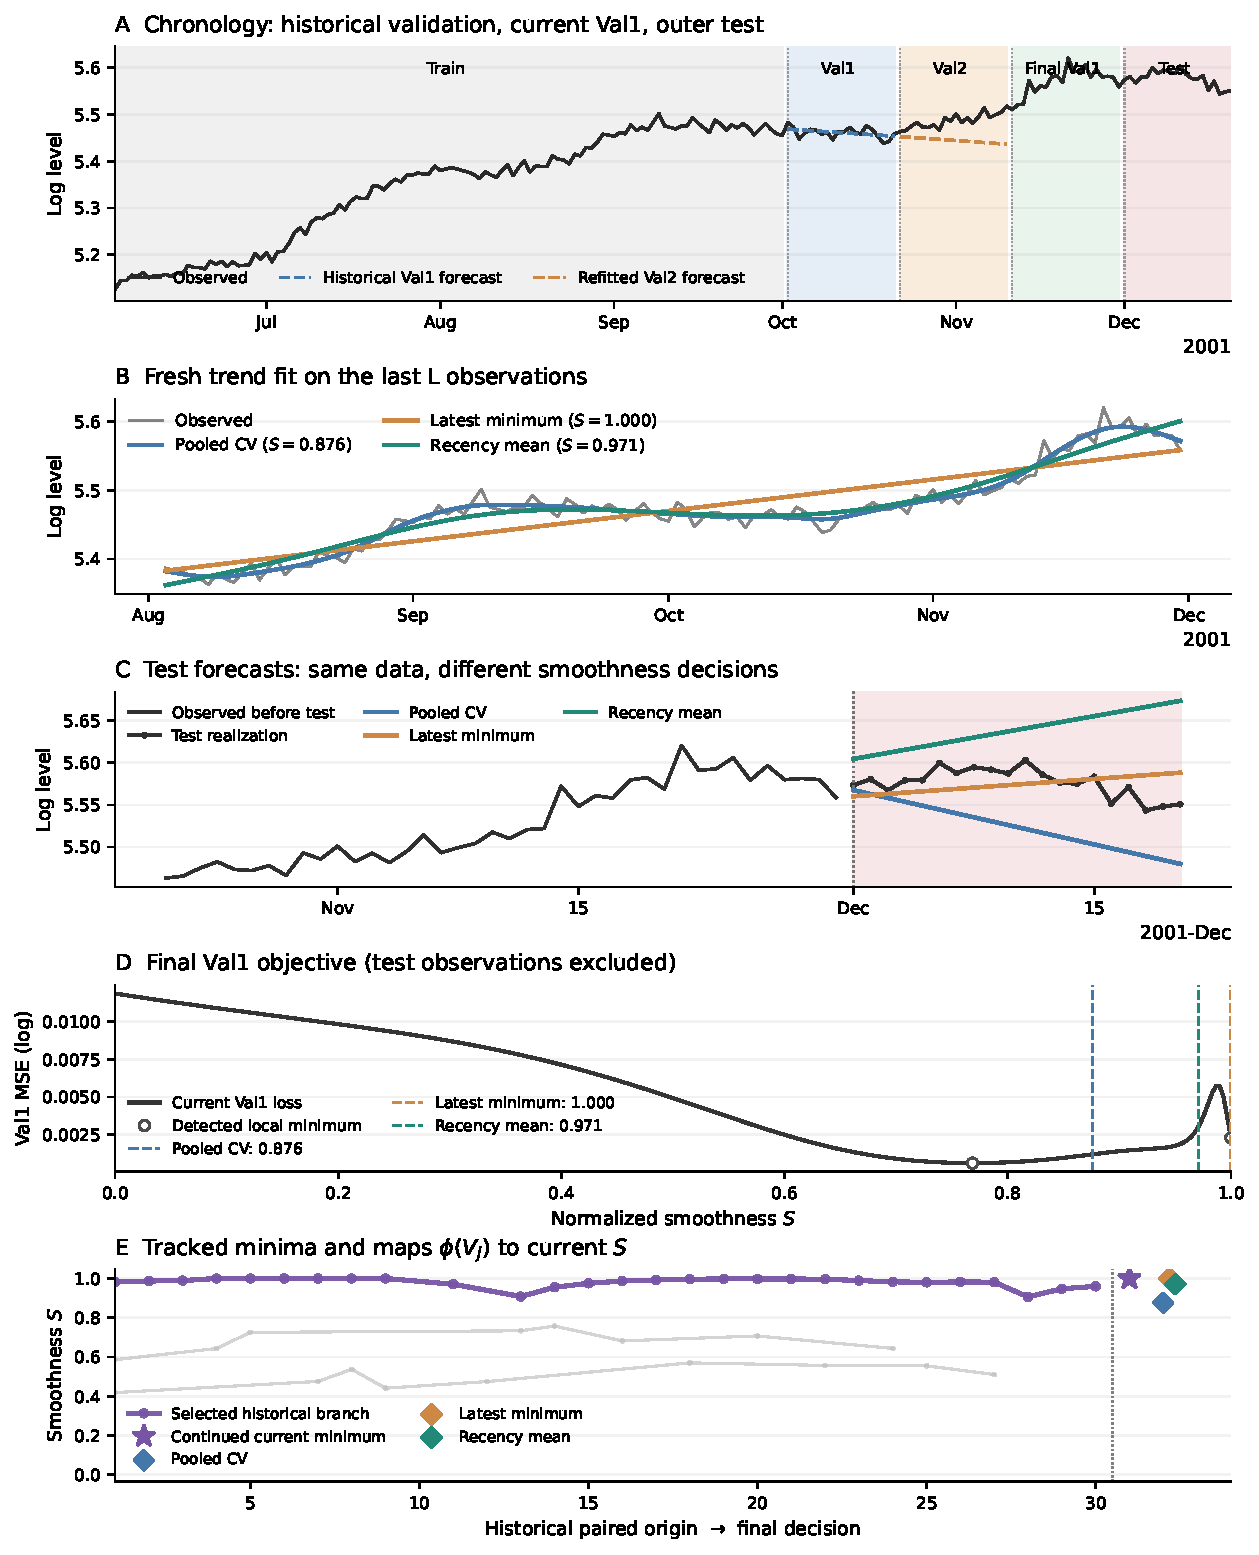
\includegraphics[
    width=\textwidth,
    height=0.73\textheight,
    keepaspectratio
]{figures/fig_workflow_tutorial.pdf}
\caption{A chronological tutorial of forecast-smoothness selection,
using the pre-specified synthetic seed 100 with a switch to roughness
($d=2$, $L=120$, $h=20$).
(A) A historical train/Validation-1/Validation-2 sequence followed by
a separate current Validation-1 block and the untouched test; the
historical Validation-2 forecast is refitted after Validation 1.
(B) New trend fits on the latest $L$ observations for pooled forecast-CV,
the newest tracked minimum, and a recency-weighted branch mean.
(C) Their multi-step test forecasts, shown with realized observations
only after selection.
(D) The \emph{current Validation-1} forecast-loss curve, its recovered
local minima, and the three smoothness choices. This is not a test-loss
curve; pooled and aggregated choices need not be minima of this surface.
(E) Historical local-minimum branches, the current continued minimum,
and final decisions $\phi(V_j)$. The illustration is pedagogical and
was not selected for favorable outer-test performance.}
\label{fig:workflow_tutorial}
\end{figure}

\subsection{Forecast performance of tracked-minimum decisions}

Checkpoint 04 evaluated branch-based smoothness selection on a small
heterogeneous panel (GDPC1, SPY, AAPL, and BTC-USD), with the recency-weighted
rule $\phi_{\mathrm{recency}}$ fixed from development data before the last four
non-overlapping test blocks per series were opened. Over the resulting 16
confirmation decisions, its geometric level-RMSE ratio was 0.692 relative to
pooled forecast-CV and 0.814 relative to the newest tracked minimum. It beat
pooled CV in 13 of 16 blocks. These are results for this particular frozen
four-series test, not a universal advantage of recency weighting.

The much broader external Checkpoint 05 panel comprised 64 previously
unused financial series (20 exchange-traded funds, 36 individual stocks, and
eight cryptocurrencies) and four test blocks per series. In these 256
decisions, the same frozen recency rule had a geometric \emph{level}-RMSE
ratio of 1.642 to pooled forecast-CV, with a descriptive series-cluster
bootstrap interval of $[1.168,\,2.703]$. Against using the newest tracked
minimum, however, its geometric ratio was 0.525. Thus smoothing the branch
trajectory substantially stabilized the newest-minimum decision in this
panel, while the pooled selector remained superior overall. The financial
series are dependent through common market shocks; the cluster interval is
a descriptive sensitivity calculation rather than an independent-series
sampling guarantee.

\subsection{The role of continuation order}

A post-hoc diagnostic of Checkpoint 05 associated extreme forecast errors
with higher-order polynomial continuation, especially the cubic
continuation induced by $d=4$. Checkpoint 06 examined that mechanism on
earlier historical blocks that did not overlap the external test blocks.
It compared successively restricted allowable difference orders,
holding the remaining branch-based protocol fixed.

The geometric level-RMSE ratios of recency weighting to pooled CV were
1.353 for $d\in\{1,2,3,4\}$, 1.200 for $\{1,2,3\}$, 1.073 for
$\{1,2\}$, and 1.045 for $d=2$ alone. Over the same order sets, the
recency/newest-minimum ratios moved from 0.691 to 0.994. The
large apparent stabilization benefit is therefore concentrated where
native higher-order continuation amplifies relatively small changes in
selected smoothness. Since the order restriction was motivated by
Checkpoint 05 outcomes, this diagnostic is explanatory, not a separately
confirmed revised forecasting method.

\subsection{Controlled changes in latent roughness}

Checkpoint 07 fixed $d=2$, $L=120$, and $h=20$ to separate changes in
smoothness from high-order continuation instability. It generated 1,200
scenarios with stationary, gradually varying, and abruptly changing
latent slope-innovation scales, and evaluated 9,600 chronological outer
forecast decisions.

The frozen recency rule yielded geometric \emph{log}-RMSE ratios to pooled
forecast-CV of 1.028 under changing roughness and 1.056 under stationary
roughness (1.037 across all mechanisms). Its ratio to the newest tracked
minimum was 0.945 overall. Hence, even under deliberately changing latent
roughness, recency averaging did not establish a general gain relative to
pooled forecast-CV. The simulation instead isolates a more modest, recurrent
property: it can damp variation in the newest-minimum rule.

\subsection{A family of smoothness decisions from the same branch}

Checkpoint 08 uses a fresh set of 100 simulation seeds with the same
controlled roughness mechanisms (1,200 scenarios, 9,600 outer decisions).
For each decision, the selected branch history is held fixed while its
final smoothness is computed by multiple functionals $\phi(V_j)$.
Examples include recency averages, least-squares extrapolations fitted
to the latest three, five, or ten branch values, exponentially weighted
linear extrapolations, and extrapolations of historical branch increments.

\Cref{tab:cp08} gives four illustrative functionals. They differ both
in observed forecasting behavior and in how frequently a raw extrapolated
smoothness lies outside the admissible interval $[0,1]$. Clipping is
unnecessary for the recency mean, since a convex average of admissible
smoothness values is itself admissible, but is needed for some forecast-based
maps. All four examples, as well as the other extrapolative rules examined
in this checkpoint, had aggregate geometric ratios above one relative to
pooled forecast-CV. They are not ranked to identify a universal winner.

\begin{table}[t]
\centering
\caption{Illustrative branch-to-smoothness functionals (Checkpoint 08).
The ratio is geometric observed-log-RMSE relative to pooled
forecast-CV; clipping refers to raw predictions outside $[0,1]$.}
\label{tab:cp08}
\begin{tabular}{@{}lcc@{}}
\toprule
Functional & RMSE ratio & Clipped (\%) \\
\midrule
Recency mean (HL 3) & 1.041 & 0.0 \\
Weighted linear (HL 5) & 1.063 & 10.8 \\
Linear extrapolation ($K=10$) & 1.079 & 18.4 \\
Weighted increments (HL 3) & 1.110 & 22.3 \\
\bottomrule
\end{tabular}
\end{table}

\Cref{fig:cp08_paths} illustrates smoothness choices from a single
fixed scenario, chosen by seed and mechanism rather than by performance.
\Cref{fig:cp08_clipping} summarizes the differing boundary behavior
of the maps. \Cref{fig:cp08_losses} displays their predictive behavior
separately for stationary and changing latent roughness. The common branch
representation supports these distinct decisions without redefining the
penalized trend estimator or carrying forward any validation-stage fitted
trend.

\begin{figure}[t]
\centering
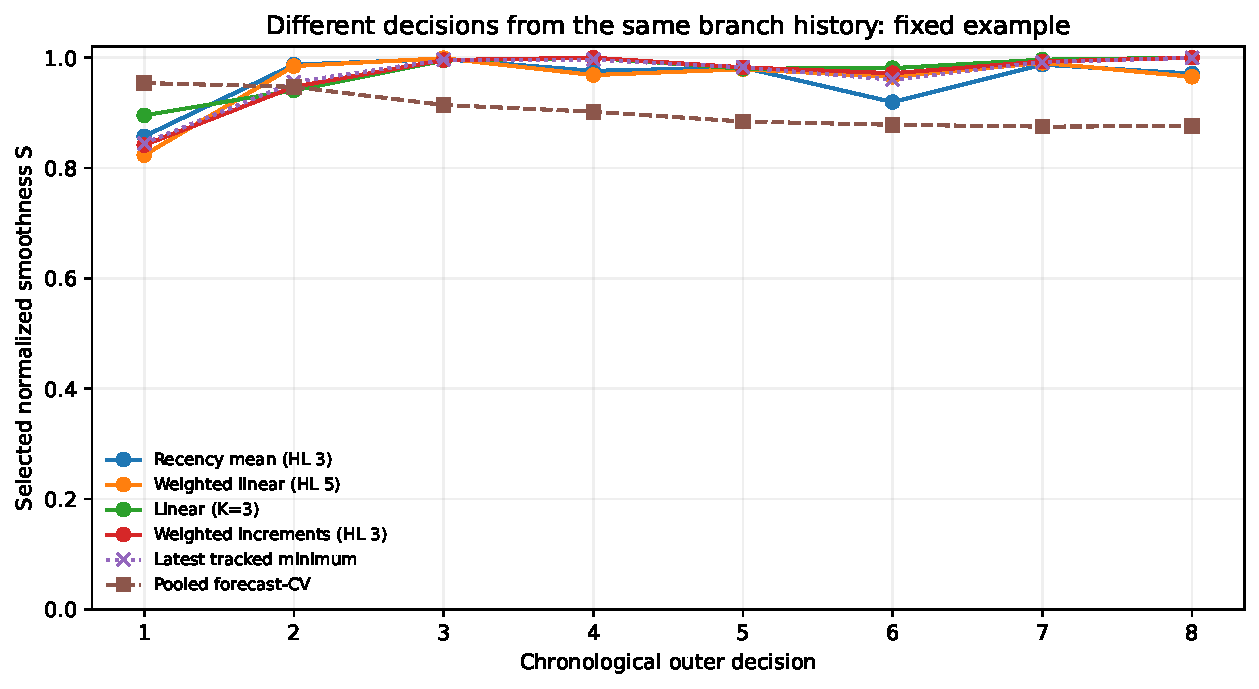
\includegraphics[width=\columnwidth]{figures/fig_cp08_illustrative_smoothness_selections.pdf}
\caption{Selected normalized smoothness across eight chronological outer
decisions under one fixed simulated roughness-switch scenario
(seed 100, noise standard deviation 0.01). The rules act on the
same recovered branch histories; the example was not selected for
favorable forecast performance.}
\label{fig:cp08_paths}
\end{figure}

\begin{figure}[t]
\centering
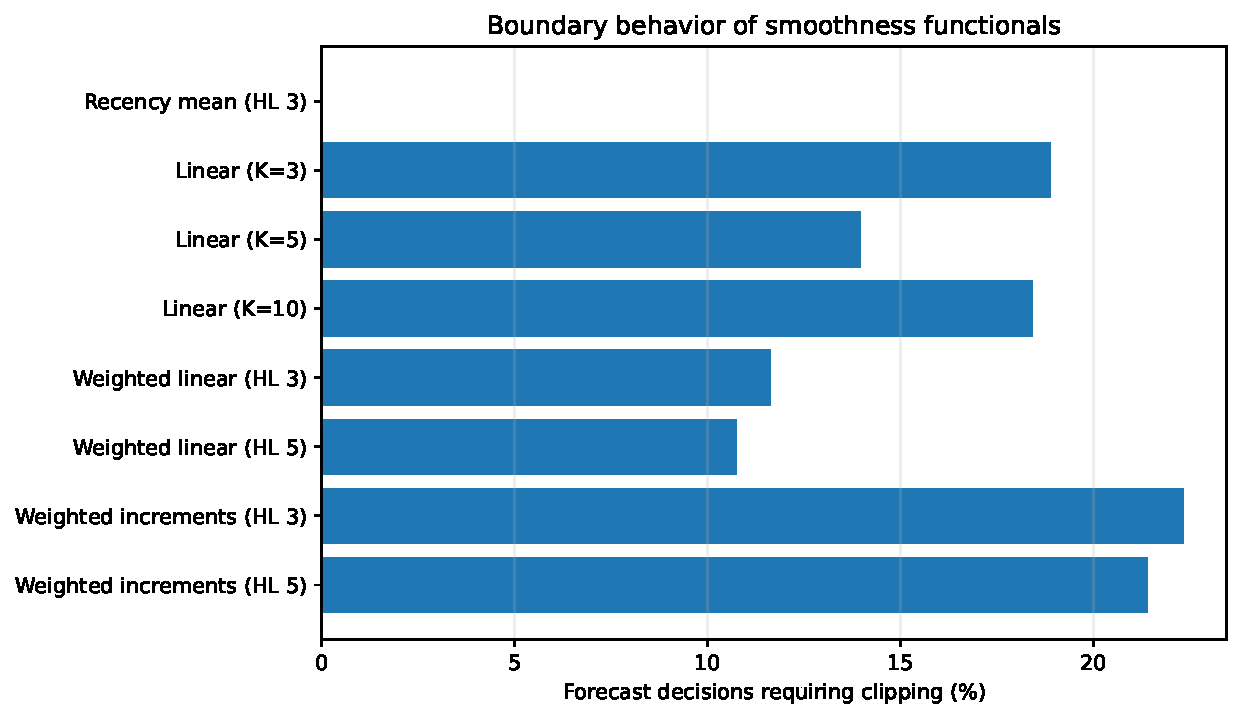
\includegraphics[width=\columnwidth]{figures/fig_cp08_rule_clipping.pdf}
\caption{Fraction of Checkpoint 08 decisions whose raw smoothness functional
requires truncation to $[0,1]$. Linear and increment extrapolations
need not preserve the interval, whereas convex recency averages do.}
\label{fig:cp08_clipping}
\end{figure}

\begin{figure}[t]
\centering
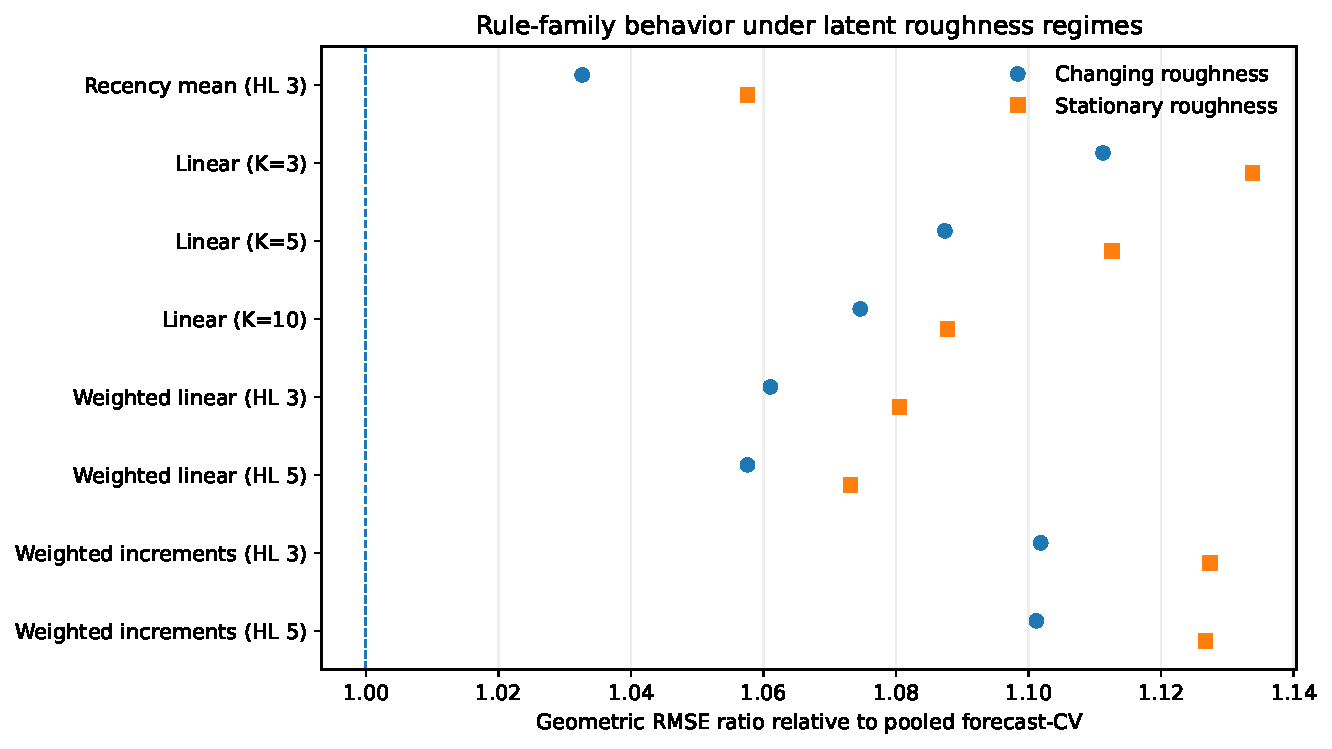
\includegraphics[width=\columnwidth]{figures/fig_cp08_rule_family_losses.pdf}
\caption{Geometric forecast-error ratios against pooled forecast-CV for
branch-to-smoothness rules in stationary and changing roughness regimes.
Values above one favor the pooled comparator. The plot describes the
behavior of a family of rules, not a data-driven winning-rule selection.}
\label{fig:cp08_losses}
\end{figure}

Together, the optional extension experiments illustrate how
historical smoothness minima may support alternative hyperparameter
choices. They do not establish that branch-based selection uniformly
improves out-of-sample forecasts, and they do not change the core
finding that horizon-matched pooled forecast-CV is a self-contained
and empirically relevant smoothness-selection procedure.
